
\documentclass[10pt]{article}
\usepackage[margin=1in]{geometry}
\usepackage{color}
\definecolor{gray}{rgb}{0.7,0.7,0.7}
\usepackage{framed}
\usepackage{enumitem}
\usepackage{longtable}
\usepackage{makecell}
\usepackage[pdfborder={0 0 0},hyperfootnotes=false]{hyperref}
\usepackage[title]{appendix}
\usepackage[calc]{picture}
\usepackage{tikz}
\usetikzlibrary{arrows}
  
\newlength{\bytewidth}
\newlength{\bytetotalheight}
\newlength{\bytedepth}
\newcommand*\byteboxsetup[1][2.1em]{\setlength{\bytewidth}{#1}
  \settototalheight{\bytetotalheight}{MQgjpqy}
  \settodepth{\bytedepth}{Qgjpqy}
  \addtolength{\bytetotalheight}{8pt}\addtolength{\bytedepth}{4pt}}

\newcommand*{\byteboxAux}[3]{\raisebox{-\bytedepth}
 {\begin{picture}(#1\bytewidth,\bytetotalheight)
    \multiput(0,0)(0,\bytetotalheight){2}{\line(1,0){#1\bytewidth}}
    #3
    \put(#1\bytewidth,0){\line(0,1){\bytetotalheight}}
    \put(0,\bytedepth){\makebox[#1\bytewidth][c]{#2}}
    \newcount\nticks \nticks #1\relax \advance\nticks -1\relax
    \multiput(\bytewidth,0)(\bytewidth,0){\nticks}{\line(0,1){3pt}}
  \end{picture}\strut}}

% Use as, e.g., \firstbytebox{2}{Tag}\bytebox{1}{\tt s}\bytebox{2}{int16\_t}
\newcommand*{\firstbytebox}[2]{\byteboxAux{#1}{#2}{\put(0,0){\line(0,1){\bytetotalheight}}}}
\newcommand*{\bytebox}[2]{\byteboxAux{#1}{#2}{}}

\newcommand*{\cclass}[1]{{\rm\sf :#1:}}
\newcommand*{\caret}{\textsuperscript{$\wedge$}}

\newcommand*{\memlimited}{\textcolor{gray}{\footnotesize\it limited}}

\begin{document}


\section{...}

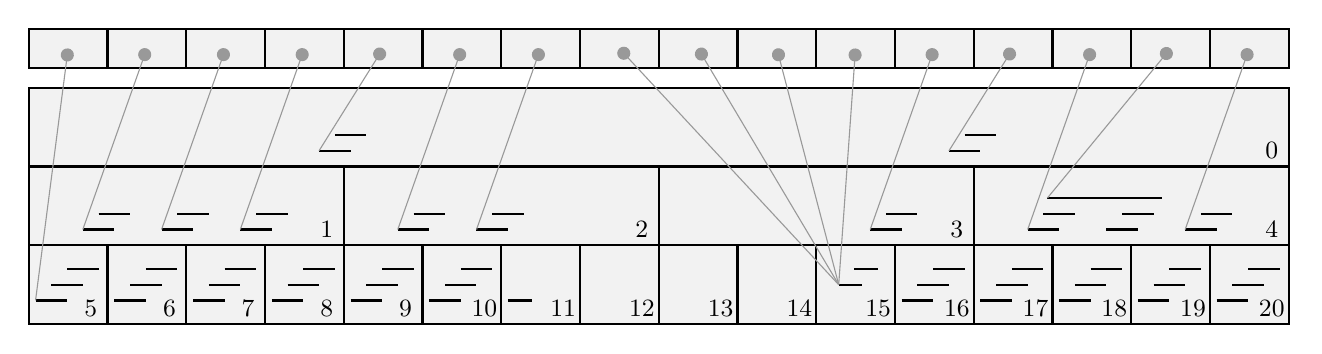
\begin{tikzpicture}
  [scale=1,
    linear/.style={rectangle, draw=black, thick, fill=black!5, minimum width=1cm, anchor=west, minimum height=0.5cm},
    block1/.style={rectangle, draw=black, thick, fill=black!5, minimum width=1cm, anchor=west, minimum height=1cm},
    block2/.style={rectangle, draw=black, thick, fill=black!5, minimum width=4cm, anchor=west, minimum height=1cm},
    block3/.style={rectangle, draw=black, thick, fill=black!5, minimum width=16cm, anchor=west, minimum height=1cm},
    line/.style={line, draw=black!20}
  ]

  \path ( 0, 4) node[linear] (l1) {}
      ++( 1, 0) node[linear] (l2) {}
      ++( 1, 0) node[linear] (l3) {}
      ++( 1, 0) node[linear] (l4) {}
      ++( 1, 0) node[linear] (l5) {}
      ++( 1, 0) node[linear] (l6) {}
      ++( 1, 0) node[linear] (l7) {}
      ++( 1, 0) node[linear] (l8) {}
      ++( 1, 0) node[linear] (l9) {}
      ++( 1, 0) node[linear] (l10){}
      ++( 1, 0) node[linear] (l11){}
      ++( 1, 0) node[linear] (l12){}
      ++( 1, 0) node[linear] (l13){}
      ++( 1, 0) node[linear] (l14){}
      ++( 1, 0) node[linear] (l15){}
      ++( 1, 0) node[linear] (l16){};

    \path ( 0, 1) node[block1] {} node at +(.8,-0.3) {\small 5}
        ++( 1, 0) node[block1] {} node at +(.8,-0.3) {\small 6}
        ++( 1, 0) node[block1] {} node at +(.8,-0.3) {\small 7}
        ++( 1, 0) node[block1] {} node at +(.8,-0.3) {\small 8}
        ++( 1, 0) node[block1] {} node at +(.8,-0.3) {\small 9}
        ++( 1, 0) node[block1] {} node at +(.8,-0.3) {\small 10}
        ++( 1, 0) node[block1] {} node at +(.8,-0.3) {\small 11}
        ++( 1, 0) node[block1] {} node at +(.8,-0.3) {\small 12}
        ++( 1, 0) node[block1] {} node at +(.8,-0.3) {\small 13}
        ++( 1, 0) node[block1] {} node at +(.8,-0.3) {\small 14}
        ++( 1, 0) node[block1] {} node at +(.8,-0.3) {\small 15}
        ++( 1, 0) node[block1] {} node at +(.8,-0.3) {\small 16}
        ++( 1, 0) node[block1] {} node at +(.8,-0.3) {\small 17}
        ++( 1, 0) node[block1] {} node at +(.8,-0.3) {\small 18}
        ++( 1, 0) node[block1] {} node at +(.8,-0.3) {\small 19}
        ++( 1, 0) node[block1] {} node at +(.8,-0.3) {\small 20}
          ( 0, 2) node[block2] {} node at +(3.8,-0.3) {\small 1}
        ++( 4, 0) node[block2] {} node at +(3.8,-0.3) {\small 2}
        ++( 4, 0) node[block2] {} node at +(3.8,-0.3) {\small 3}
        ++( 4, 0) node[block2] {} node at +(3.8,-0.3) {\small 4}
          ( 0, 3) node[block3] {} node at +(15.8,-0.3) {\small 0};

        % layer 1
        \foreach \b in {0,1,2,3,4,5,  11,12,13,14,15} {
          \foreach \x in {0,1,2} {
            \draw[thick] (\b.1+\x/5, 0.8+\x/5) coordinate (r1_\b_\x)
                      -- (\b.5+\x/5, 0.8+\x/5);
          }
        }
        \draw[thick] (6.1,  0.8+0/5) -- (6.4,  0.8+0/5);
        \draw[thick] (10.3, 0.8+1/5) coordinate (r1_10_0) -- (10.6, 0.8+1/5);
        \draw[thick] (10.5, 0.8+2/5) -- (10.8, 0.8+2/5);

        % layer 2
        \foreach \b in {0,1,2, ,4,5,  10,  12,13,14} {
          \foreach \x in {0,1} {
            \draw[thick] (\b+.7+\x/5,  1.7+\x/5) coordinate (r2_\b_\x)
                      -- (\b+1.1+\x/5, 1.7+\x/5);
          }
        }

        % layer3
        \foreach \b in {3, 11} {
          \foreach \x in {0,1} {
            \draw[thick] (\b+.7+\x/5,  2.7+\x/5) coordinate (r3_\b_\x)
                      -- (\b+1.1+\x/5, 2.7+\x/5);
          }
        }
        \draw[thick] (12.95,2.1) coordinate (r2_12_2) -- (14.4,2.1);

        \draw [>=*,<-,black!40](l1.center)  -- (r1_0_0.west);
        \draw [>=*,<-,black!40](l2.center)  -- (r2_0_0.west);
        \draw [>=*,<-,black!40](l3.center)  -- (r2_1_0.west);
        \draw [>=*,<-,black!40](l4.center)  -- (r2_2_0.west);
        \draw [>=*,<-,black!40](l5.center)  -- (r3_3_0.west);
        \draw [>=*,<-,black!40](l6.center)  -- (r2_4_0.west);
        \draw [>=*,<-,black!40](l7.center)  -- (r2_5_0.west);
        \draw [>=*,<-,black!40](l8.center)  -- (r1_10_0.west);
        \draw [>=*,<-,black!40](l9.center)  -- (r1_10_0.west);
        \draw [>=*,<-,black!40](l10.center) -- (r1_10_0.west);
        \draw [>=*,<-,black!40](l11.center) -- (r1_10_0.west);
        \draw [>=*,<-,black!40](l12.center) -- (r2_10_0.west);
        \draw [>=*,<-,black!40](l13.center) -- (r3_11_0.west);
        \draw [>=*,<-,black!40](l14.center) -- (r2_12_0.west);
        \draw [>=*,<-,black!40](l15.center) -- (r2_12_2.west);
        \draw [>=*,<-,black!40](l16.center) -- (r2_14_0.west);

\end{tikzpicture}

% \begin{tikzpicture}[
%     thick, xscale=2, yscale=1.8,
%     read/.style={line width=0.4mm},
%     block/.style={rectangle, width=0.2mm},
%   ]
% 
% \draw (0,0) node[block] (C) {b1};
% \end{tikzpicture}

\end{document}
